% 来源：固定来源 PDF（2004福建文.pdf）第 1 页（印刷页 166）Q16 正六棱柱折纸展开图
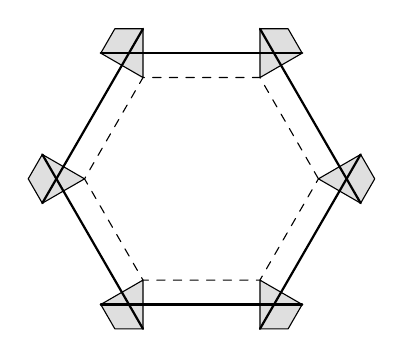
\begin{tikzpicture}[scale=1.1, line cap=round, line join=round]
  \tikzset{
    outer/.style={thick},
    fold/.style={dashed, thin},
    cutout/.style={fill=gray!25, draw=black, thin}
  }

  % 参数：外半径 R=2.0，内半径 r=1.35
  \def\R{2.0}
  \def\r{1.35}

  % 计算切角并填充六个角处的四边形阴影
  \foreach \i in {0, 1, ..., 5} {
    \pgfmathsetmacro{\ang}{\i * 60}
    \pgfmathsetmacro{\prevang}{(\i - 1) * 60}
    \pgfmathsetmacro{\nextang}{(\i + 1) * 60}

    % 外顶点 V
    \coordinate (V\i) at ({\R * cos(\ang)}, {\R * sin(\ang)});
    % 内顶点 W
    \coordinate (W\i) at ({\r * cos(\ang)}, {\r * sin(\ang)});

    % 两侧切口点（从 W 向相邻外边作垂线的垂足）
    \pgfmathsetmacro{\angA}{\ang + 30}
    \pgfmathsetmacro{\dist}{0.5 * (\R - \r)}
    \coordinate (P\i) at ({\R * cos(\ang) - \dist * cos(\ang - 60)}, {\R * sin(\ang) - \dist * sin(\ang - 60)});
    \coordinate (Q\i) at ({\R * cos(\ang) - \dist * cos(\ang + 60)}, {\R * sin(\ang) - \dist * sin(\ang + 60)});

    \filldraw[cutout] (W\i) -- (P\i) -- (V\i) -- (Q\i) -- cycle;
  }

  % 外边界未切除边段
  \foreach \i in {0, 1, ..., 5} {
    \pgfmathsetmacro{\nexti}{int(mod(\i + 1, 6))}
    \draw[outer] (Q\i) -- (P\nexti);
  }

  % 内部虚线折痕（内正六边形）
  \draw[fold] (W0) -- (W1) -- (W2) -- (W3) -- (W4) -- (W5) -- cycle;
\end{tikzpicture}
